% !TEX encoding = UTF-8 Unicode
%!TEX TS-program = xelatex

\documentclass[12pt]{extarticle}
% extarticle is like article but can handle 8pt, 9pt, 10pt, 11pt, 12pt, 14pt, 17pt, and 20pt text

\def \ititle {Origins of Mind}
 
\def \isubtitle {Lecture 08}
 
\def \iauthor {Stephen A. Butterfill}
\def \iemail{s.butterfill@warwick.ac.uk}
\date{}

%for strikethrough
\usepackage[normalem]{ulem}

\usepackage{pdfpages}


\input{$HOME/Documents/submissions/preamble_steve_handout}

%logic symbol \leftmodels
\usepackage{MnSymbol}

%\bibpunct{}{}{,}{s}{}{,}  %use superscript TICS style bib
%remove hanging indent for TICS style bib
%TODO doesnt work
\setlength{\bibhang}{0em}
%\setlength{\bibsep}{0.5em}


%itemize bullet should be dash
\renewcommand{\labelitemi}{$-$}

\begin{document}

%\raggedcolumns

\begin{multicols*}{3}

\setlength\footnotesep{1em}


\bibliographystyle{newapa} %apalike

%\maketitle
%\tableofcontents




%--------------- 
%--- start paste


\def \ititle {Logic I}
 
\def \isubtitle {Lecture 08}
 
\begin{center}
 
{\Large
 
\textbf{\ititle}: \isubtitle
 
}
 
 
 
\iemail %
 
\end{center}
 
Readings refer to sections of the course textbook, \emph{Language, Proof and Logic}.
 
 
 
\section{Everything Is Broken}
 
\emph{Reading:} §9.1, §9.2
 
Everything is broken: ∀x Broken(x)
 
Something is broken: ∃x Broken(x)
 
 
 
\section{All Squares Are Blue}
 
\emph{Reading:} §9.2, §9.3, §9.5
 
 
 
\section{What does ∀ mean?}
 
\emph{Reading:} §9.4
 
We give the meaning of ∀ by specifying what it takes for a sentence containing ∀ to be true:
 
\begin{enumerate}
 
\item Give every object a name.
 
\item For each name in turn, create a new sentence like this: delete the quantifier and replace all instances of the variable it binds with that name.
 
\item If ALL of the new sentences are true, so is the original sentence.
 
\end{enumerate}
 
 
 
\section{Vegetarians Are Evil}
 
\emph{Reading:} §9.2, §9.3, §9.5
 
\begin{center}
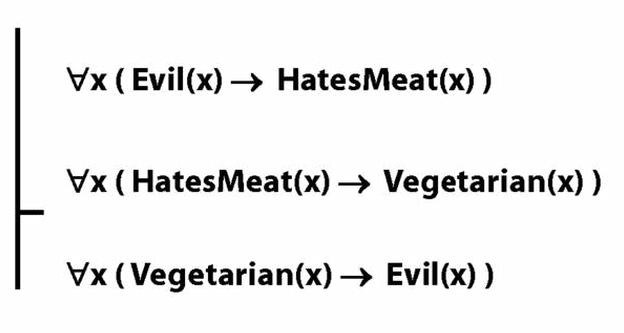
\includegraphics[scale=0.3]{img/vegetarians.png}
\end{center}
 
 
\section{Not If}
 
\begin{center}
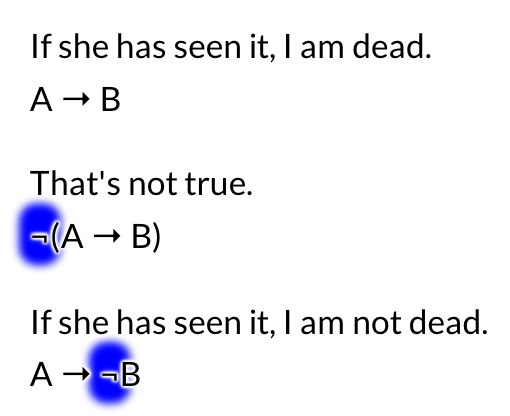
\includegraphics[scale=0.3]{img/not_if.png}
\end{center}
\begin{center}
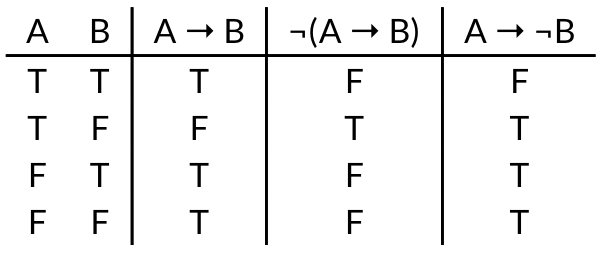
\includegraphics[scale=0.3]{img/not_if_tt.png}
\end{center}
 
 
\section{Scope: A Mistaken Application of ¬Elim}
 
What is wrong with this proof?
 
\begin{center}
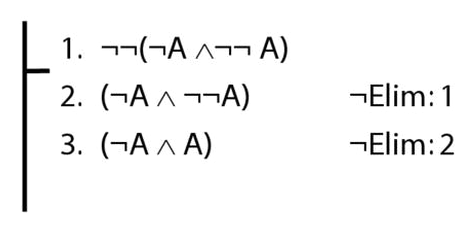
\includegraphics[scale=0.3]{img/proof_negation_elim_wrong.png}
\end{center}
 
 
\section{Scope}
 
\emph{Reading:} §3.5
 
The \emph{scope} of a connective (token) is the sentence containing it lowest in the tree.
 
\begin{center}
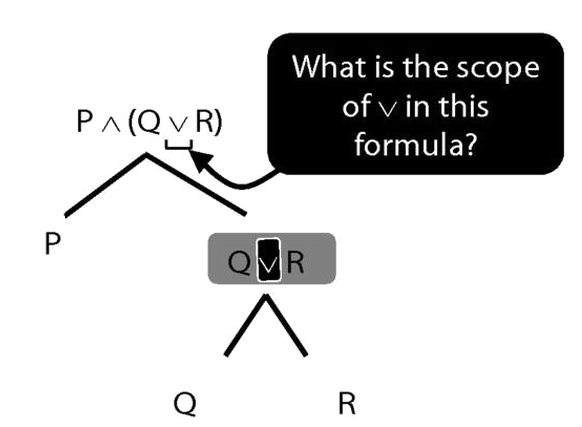
\includegraphics[scale=0.3]{img/unit_290_scope_q.png}
\end{center}
The connective with \emph{widest scope} is the one whose scope is the whole sentence.
 
\begin{center}
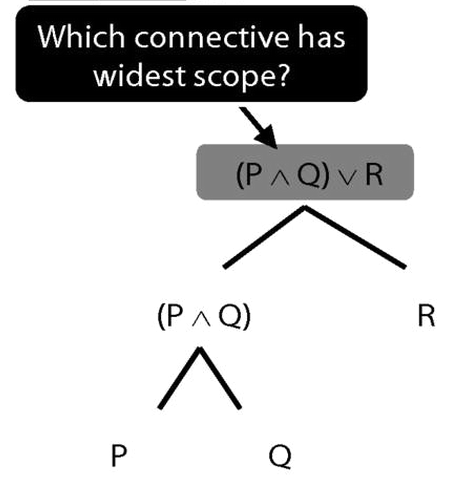
\includegraphics[scale=0.3]{img/unit_290_scope_q2.png}
\end{center}
A rule of proof can only be applied to the connective with widest scope.
 
\begin{center}
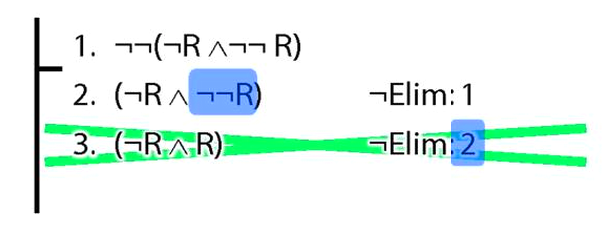
\includegraphics[scale=0.3]{img/unit_290_scope_proof.png}
\end{center}
When we do truth tables, the order we do the columns in is determined by scope.
 
\begin{center}
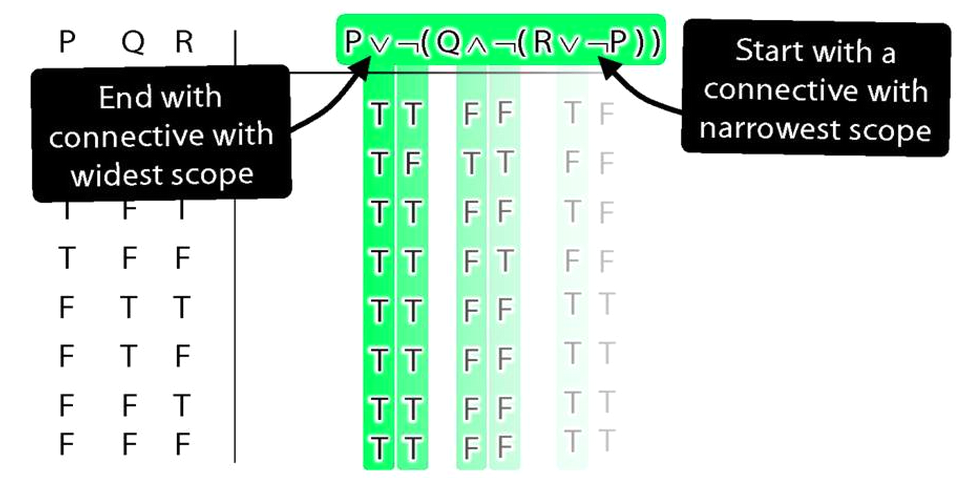
\includegraphics[scale=0.3]{img/unit_290_scope_tt.png}
\end{center}
 
 
\section{Proof Example: ¬(P∨Q) therefore ¬P∧¬Q}
 
\begin{center}
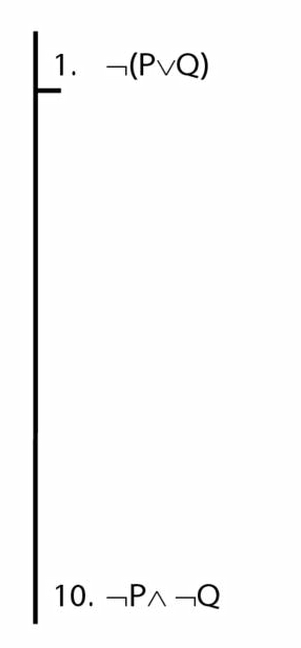
\includegraphics[scale=0.3]{img/unit_821_proof.png}
\end{center}
\begin{center}
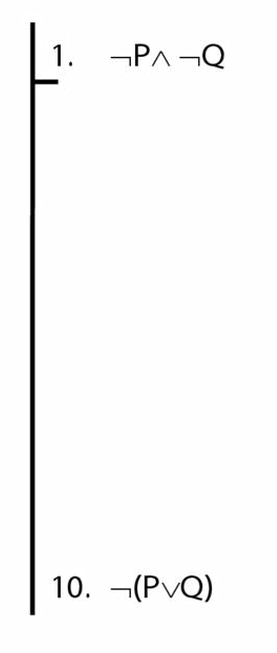
\includegraphics[scale=0.3]{img/unit_821_proof2.png}
\end{center}
 


%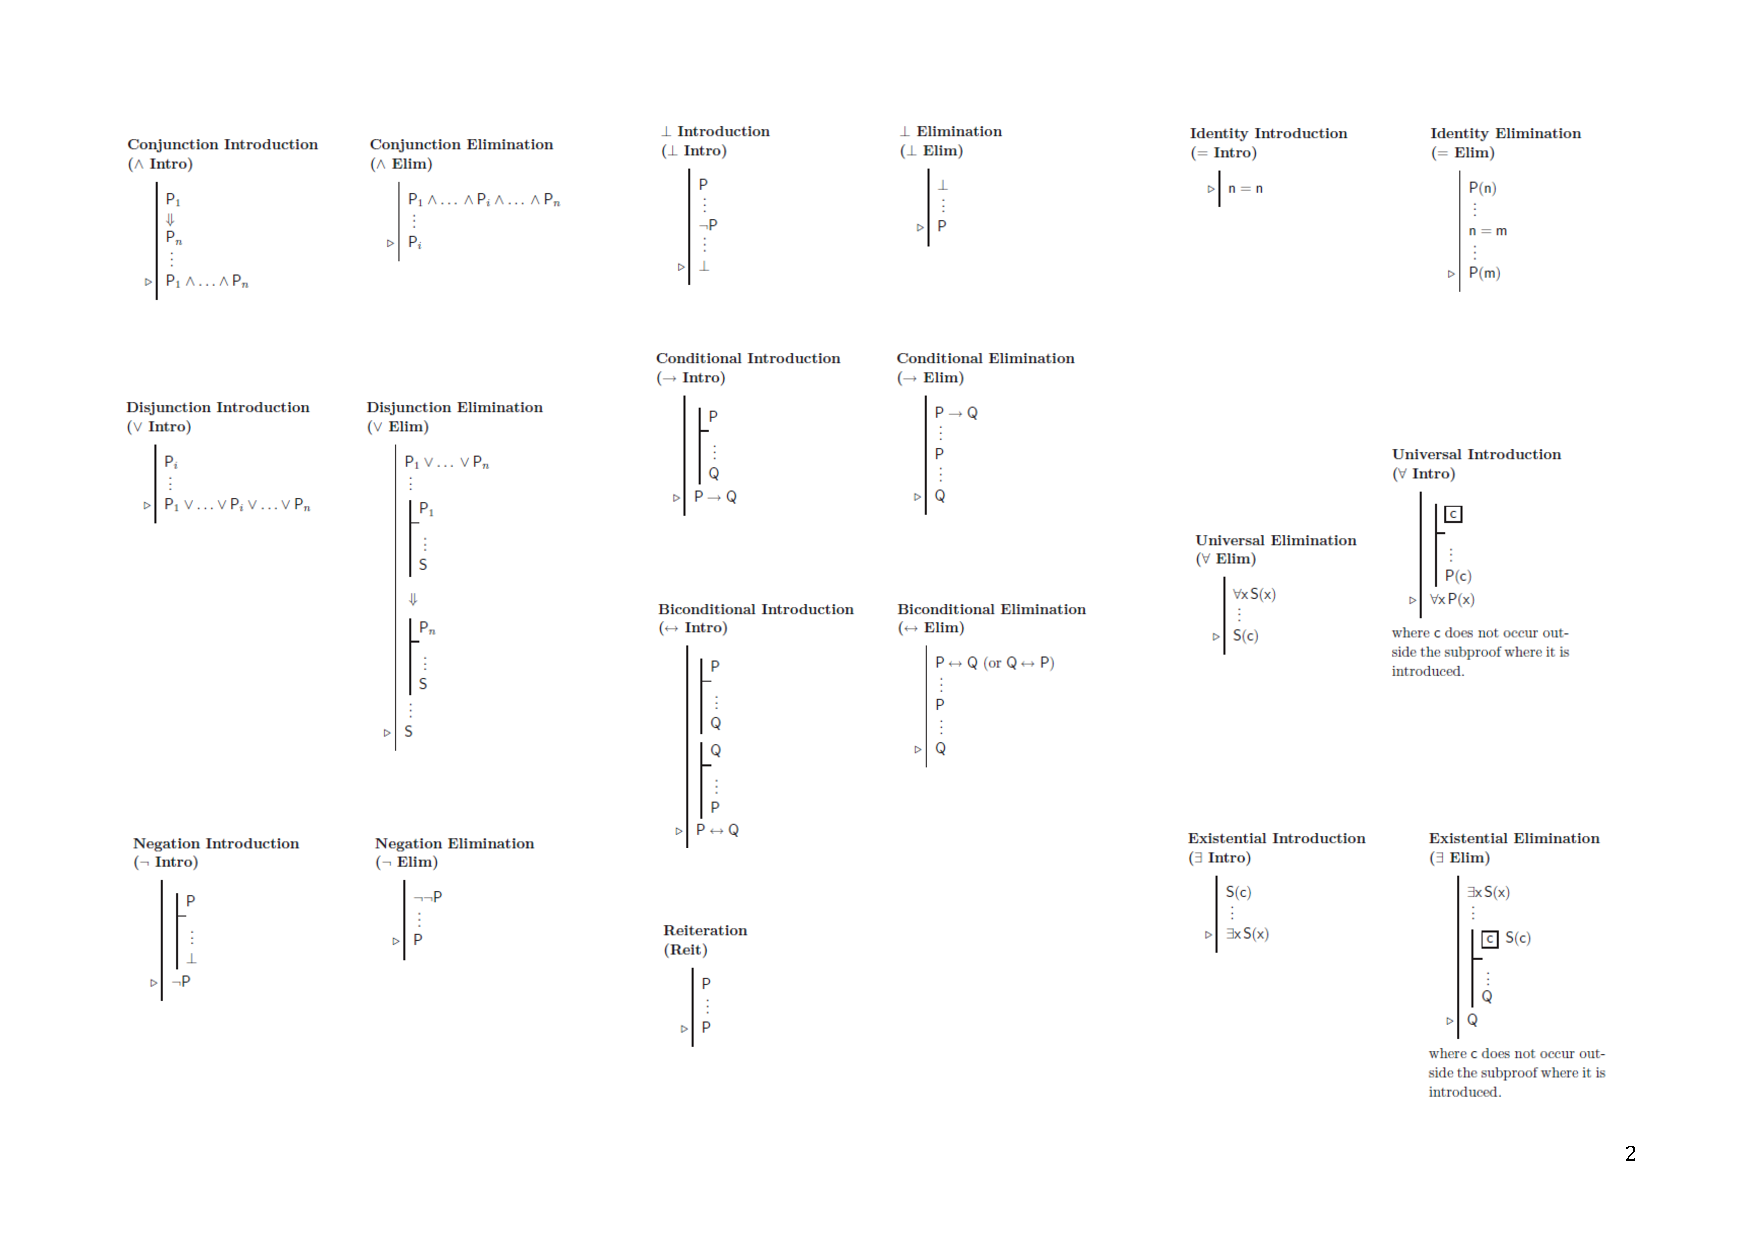
\includepdf[pages={1}]{img/rules.pdf}
 

%--- end paste
%--------------- 
 


\end{multicols*}

\end{document}